% SIAM Supplemental File Template
\documentclass[review,supplement,hidelinks,onefignum,onetabnum]{siamart220329}

\usepackage[utf8]{inputenc}
\usepackage{tikz}
\usepackage{dot2texi}
\usetikzlibrary{arrows,positioning}
\usepackage{subcaption}

\begin{document}

\title{Digraph Arborescences and Matrix Determinants}
\author{Sayani Ghosh\thanks{Department of Physics and Astronomy, Clemson University, Clemson, SC 29634 ({\email{sayanig@g.clemson.edu}})} \and Bradley S. Meyer\thanks{Department of Physics and Astronomy, Clemson University, Clemson, SC 29634
({\email{mbradle@g.clemson.edu})}}}

\maketitle

\section{Matrix-Tree Example}
Consider the $3 \times 3$ matrix
\begin{equation}
    A = \begin{pmatrix}
v_{11} + v_{21} + v_{31} & -v_{12} & -v_{13}\\
-v_{21} & v_{22} + v_{12} + v_{32} & -v_{23} \\
-v_{31}  & -v_{32}& v_{13} + v_{23} + v_{33}
\end{pmatrix}
\label{eq:A}
\end{equation}
The matrix digraph for $A$ is shown in Fig. \ref{fig:3digraph}. The resulting determinant is
\begin{equation}
\begin{split}
    det(A) &= v_{11} v_{22} v_{33} + v_{11} v_{22} v_{13} + v_{11} v_{22} v_{23} + v_{11} v_{12} v_{13} \\
    &+ v_{11} v_{12} v_{23} + v_{11} v_{12} v_{33}
    + v_{11} v_{32} v_{13} + v_{11} v_{32} v_{33} \\
    &+ v_{21} v_{22} v_{13} + v_{21} v_{22} v_{23} + v_{21} v_{22} v_{33} + v_{31} v_{22} v_{23} \\
    &+ v_{31} v_{22} v_{33} + v_{31} v_{12} v_{33} + v_{31} v_{32} v_{33} + v_{21} v_{32} v_{33}
\end{split}
\label{eq:example_det}
\end{equation}
which arises from the sum over the 16 arborescences possible in the digraph in Fig. \ref{fig:3digraph}.

\begin{center}
\begin{figure}[h]
\centering
    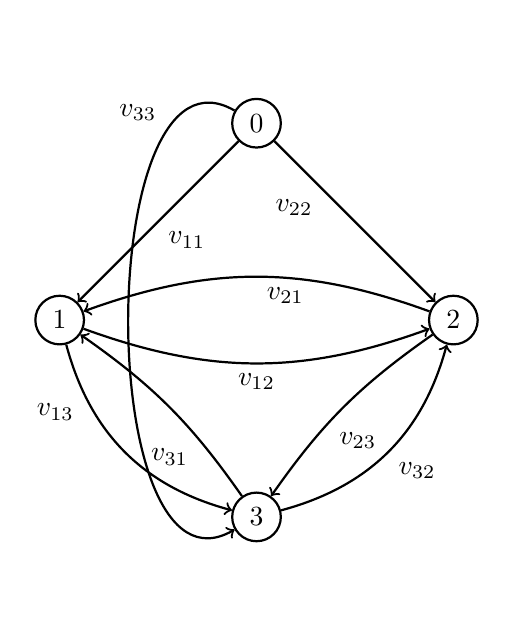
\begin{tikzpicture}[node distance={40mm}, thick, main/.style = {draw, circle}] 
    \node[main] (1) at (0,0) {$0$};
    \node[main] (2) at (-2.5,-2.5) {$1$};
    \node[main] (3) at ( 2.5,-2.5) {$2$};
    \node[main] (4) at (0,-5) {$3$};

    \draw[->] (1) -- node[midway, below right]{$v_{11}$} (2);
    \draw[->] (1) -- node[midway, below left, pos = 0.3]{$v_{22}$} (3);
    \draw[->] (1) edge [bend right = 120] node[midway, above left, pos =0.2]{$v_{33}$} (4);

    \draw[->, black] (2) edge [bend right = 20] node [left, below] {$v_{12}$} (3);
    \draw[->, black] (3) edge [bend right = 20] node [left, below right] {$v_{21}$} (2);
    \draw[->, black] (2) edge [bend right] node [right, below left, pos = 0.2] {$v_{13}$} (4);
    \draw[->, black] (4) edge [bend right = 10] node [left, below left, pos = 0.3] {$v_{31}$} (2);
    \draw[->, black] (4) edge [bend right] node [left, below right] {$v_{32}$} (3);
    \draw[->, black] (3) edge [bend right = 10] node [left, below right, pos = 0.6] {$v_{23}$} (4);

    \end{tikzpicture} 
    \caption{A $3$-vertex digraph with root vertex 0.} \label{fig:3digraph}
\end{figure}
\end{center}
    
    \section{Modified Reduced Matrix Example}
    Consider the matrix
\begin{equation}
    A' = \begin{pmatrix}
v_{11} + v_{21} + v_{31} & -v_{12} & 1 \\
-v_{21} & v_{22} + v_{12} + v_{32} & 1 \\
-v_{31}  & -v_{32}& 0
\end{pmatrix}
\end{equation}
derived from Eq. (\ref{eq:A}).  This matrix
can be written
\begin{equation}
A' = \begin{pmatrix}
v_{11} + v_{21} + v_{31} & -v_{12} & 0 \\
-v_{21} & v_{22} + v_{12} + v_{32} & 0 \\
-v_{31}  & -v_{32}& 0
\end{pmatrix}
+
\begin{pmatrix}
0 & 0 & 1 \\
0 & 0 & 0 \\
0 & 0 & 0
\end{pmatrix}
+
\begin{pmatrix}
0 & 0 & 0 \\
0 & 0 & 1 \\
0 & 0 & 0
\end{pmatrix}
\label{eq:mod1}
\end{equation}
The determinant of $A$ is the sum of determinants of matrices made up of the various permutations of columns of $A'$.  Thus,
\begin{equation}
\begin{split}
det(A') &= det\begin{pmatrix}
v_{11} + v_{21} + v_{31} & -v_{12} & 1 \\
-v_{21} & v_{22} + v_{12} + v_{32} & 0 \\
-v_{31}  & -v_{32}& 0
\end{pmatrix} \\
&+ 
det\begin{pmatrix}
v_{11} + v_{21} + v_{31} & -v_{12} & 0 \\
-v_{21} & v_{22} + v_{12} + v_{32} & 1 \\
-v_{31}  & -v_{32}& 0
\end{pmatrix} \\
&= det(A^{\{1\},\{3\}}) + det(A^{\{2\},\{3\}})
\end{split}
\label{eq:mod2}
\end{equation}
Other permuted matrices in the sum yield zero determinant, so the surviving terms will be determinants of reduced matrices.

    \section{Factoring Example}  \label{append:factoring}

Consider the matrix digraph in Fig. \ref{fig:3digraph}.  To factor the determinant of the corresponding matrix (Eq. (\ref{eq:A})), first create a digraph $\Gamma_1$ that is explicitly rooted at vertex $1$ and a digraph ${\bar \Gamma}_1$ that is explicitly not rooted at vertex $1$.  $\Gamma_1$ is shown in Fig. \ref{fig:g1}(a).  Then isolate vertex $1$ by moving the arcs $(1,2)$ and $(1,3)$ to $(0, 2)$ and $(0, 3)$, respectively, and combining with the existing arcs.  This results in the digraph in Fig. \ref{fig:g1}(b).

\begin{figure}[htb!]
\centering 
  \begin{subfigure}[b]{0.25\textwidth}
  \centering
    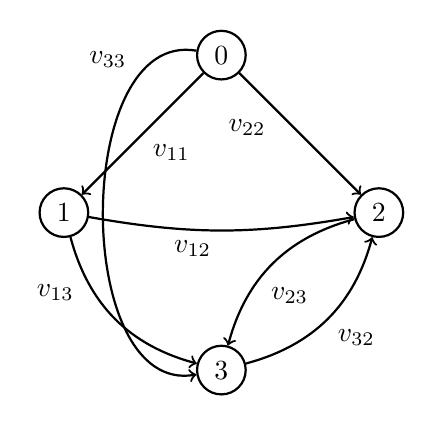
\begin{tikzpicture}[node distance={10mm}, thick, main/.style = {draw, circle}] 
    \node[main] (1) at (0,0) {$0$};
    \node[main] (2) at (-2,-2) {$1$};
    \node[main] (3) at ( 2,-2) {$2$};
    \node[main] (4) at (0,-4) {$3$};

    \draw[->] (1) -- node[midway, below right]{$v_{11}$} (2);
    \draw[->] (1) -- node[midway, below left, pos = 0.3]{$v_{22}$} (3);
    \draw[->] (1) edge [bend right = 100] node[midway, above left, pos =0.2]{$v_{33}$} (4);

    \draw[->] (2) edge [bend right = 10] node [midway, below left] {$v_{12}$} (3);
    \draw[->, black] (2) edge [bend right] node [right, below left, pos = 0.2] {$v_{13}$} (4);
    \draw[->, black] (4) edge [bend right] node [left, below right] {$v_{32}$} (3);
    \draw[->, black] (3) edge [bend right] node [left, below right, pos = 0.6] {$v_{23}$} (4);
    \end{tikzpicture} 
    \caption{$\Gamma_1$ before isolation.}
  \end{subfigure} 
  \hspace{6em}
  \begin{subfigure}[b]{0.25\textwidth}
  \centering
    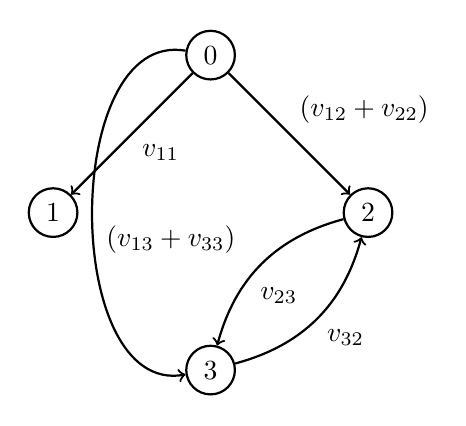
\begin{tikzpicture}[node distance={10mm}, thick, main/.style = {draw, circle}] 
    \node[main] (1) at (0,0) {$0$};
    \node[main] (2) at (-2,-2) {$1$};
    \node[main] (3) at ( 2,-2) {$2$};
    \node[main] (4) at (0,-4) {$3$};

    \draw[->] (1) -- node[midway, below right]{$v_{11}$} (2);
    \draw[->] (1) -- node[midway, above right]{$(v_{12}+v_{22})$} (3);
    \draw[->] (1) edge [bend right = 100] node[midway, above right, pos = 0.6]{$(v_{13}+v_{33})$} (4);

    \draw[->, black] (4) edge [bend right] node [left, below right] {$v_{32}$} (3);
    \draw[->, black] (3) edge [bend right] node [left, below right, pos = 0.6] {$v_{23}$} (4);
    \end{tikzpicture} 
    \caption{$\Gamma_1$ after isolation.}
    \end{subfigure}

    \caption{Digraph $\Gamma_1$ explicitly rooted at vertex $1$.}\label{fig:g1}
\end{figure}

Next, explicitly root the digraph in Fig. \ref{fig:g1} at vertex $2$ to obtain the digraph $\Gamma_{1,2}$ and isolate vertex $2$ in that digraph to obtain the fully isolated digraph in Fig. \ref{fig:g1_23}(a).  Similarly explicitly root the digraph in Fig. \ref{fig:g1} at vertex $3$ to obtain the fully isolated digraph in Fig. \ref{fig:g1_23}(b).

\begin{figure}[htb!]
\centering 
  \begin{subfigure}[b]{0.25\textwidth}
  \centering
    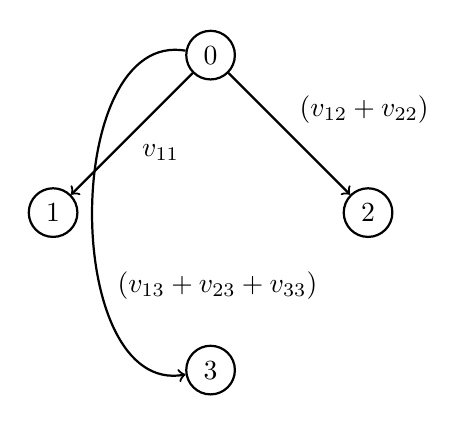
\begin{tikzpicture}[node distance={10mm}, thick, main/.style = {draw, circle}] 
    \node[main] (1) at (0,0) {$0$};
    \node[main] (2) at (-2,-2) {$1$};
    \node[main] (3) at ( 2,-2) {$2$};
    \node[main] (4) at (0,-4) {$3$};

    \draw[->] (1) -- node[midway, below right]{$v_{11}$} (2);
    \draw[->] (1) -- node[midway, above right]{$(v_{12}+v_{22})$} (3);
    \draw[->] (1) edge [bend right = 100] node[midway, above right, pos = 0.7]{$(v_{13}+v_{23}+v_{33})$} (4);
    \end{tikzpicture} 
    \caption{$\Gamma_{1,2}$ after isolation.}  
  \end{subfigure} 
  \hspace{6em}
  \begin{subfigure}[b]{0.25\textwidth}
  \centering
    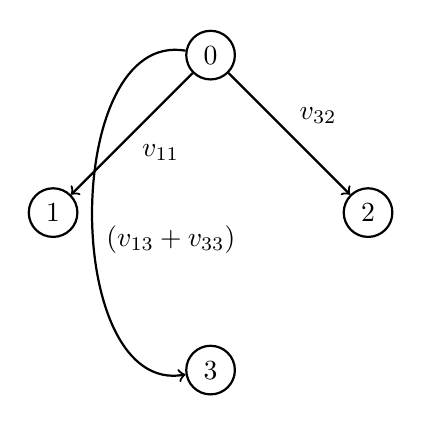
\begin{tikzpicture}[node distance={10mm}, thick, main/.style = {draw, circle}] 
    \node[main] (1) at (0,0) {$0$};
    \node[main] (2) at (-2,-2) {$1$};
    \node[main] (3) at ( 2,-2) {$2$};
    \node[main] (4) at (0,-4) {$3$};

    \draw[->] (1) -- node[midway, below right]{$v_{11}$} (2);
    \draw[->] (1) -- node[midway, above right]{$v_{32}$} (3);
    \draw[->] (1) edge [bend right = 100] node[midway, above right, pos = 0.6]{$(v_{13}+v_{33})$} (4);

    \end{tikzpicture} 
    \caption{$\Gamma_{1,3}$ after isolation.}
    \end{subfigure}

    \caption{Fully isolated $\Gamma_1$ digraphs.  (a) $W(B) = v_{11}(v_{12}+v_{22})(v_{13}+v_{23}+v_{33})$. (b) $W(B) = v_{11}v_{32}(v_{13}+v_{33})$.}
\label{fig:g1_23}
\end{figure}

Now return to ${\bar \Gamma}_1$, which is not rooted at vertex $1$.  From that digraph create a digraph $\Gamma_2$ explicitly rooted at vertex $2$ and digraph ${\bar \Gamma}_2$, which is explicitly not rooted at vertex $2$.  For this example, ${\bar \Gamma}_2$ is explicitly only rooted at vertex $3$, so ${\bar \Gamma}_2 = \Gamma_3$.  Follow the isolation procedure on $\Gamma_2$ to obtain the fully isolated digraphs in Fig. \ref{fig:g2}.

\begin{figure}[htb!]
\centering 
  \begin{subfigure}[b]{0.25\textwidth}
  \centering
    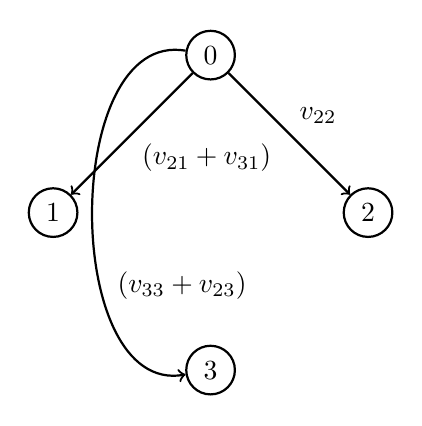
\begin{tikzpicture}[node distance={10mm}, thick, main/.style = {draw, circle}] 
    \node[main] (1) at (0,0) {$0$};
    \node[main] (2) at (-2,-2) {$1$};
    \node[main] (3) at ( 2,-2) {$2$};
    \node[main] (4) at (0,-4) {$3$};

    \draw[->] (1) -- node[midway, below right]{$(v_{21}+v_{31})$} (2);
    \draw[->] (1) -- node[midway, above right]{$v_{22}$} (3);
    \draw[->] (1) edge [bend right = 100] node[midway, above right, pos = 0.7]{$(v_{33} + v_{23})$} (4);
    \end{tikzpicture} 
    \caption{$\Gamma_{2,1}$ after isolation.}
  \end{subfigure} 
  \hspace{6em}
  \begin{subfigure}[b]{0.25\textwidth}
  \centering
    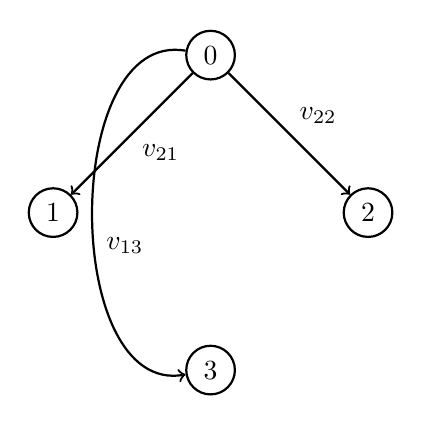
\begin{tikzpicture}[node distance={10mm}, thick, main/.style = {draw, circle}] 
    \node[main] (1) at (0,0) {$0$};
    \node[main] (2) at (-2,-2) {$1$};
    \node[main] (3) at ( 2,-2) {$2$};
    \node[main] (4) at (0,-4) {$3$};

    \draw[->] (1) -- node[midway, below right]{$v_{21}$} (2);
    \draw[->] (1) -- node[midway, above right]{$v_{22}$} (3);
    \draw[->] (1) edge [bend right = 100] node[midway, above right, pos = 0.6]{$v_{13}$} (4);

    \end{tikzpicture} 
    \caption{$\Gamma_{2,3}$ after isolation.} 
    \end{subfigure}

    \caption{Fully isolated $\Gamma_2$ digraphs.  (a) $W(B) = (v_{21}+v_{31})(v_{22})(v_{33} + v_{23})$. (b) $W(B) =v_{21}v_{22}v_{13}$.}\label{fig:g2}
\end{figure}

Similarly follow the isolation procedure for $\Gamma_3$ to obtain the digraphs in Fig. \ref{fig:g3}.

\begin{figure}[t!]
\centering 
  \begin{subfigure}[b]{0.25\textwidth}
  \centering
    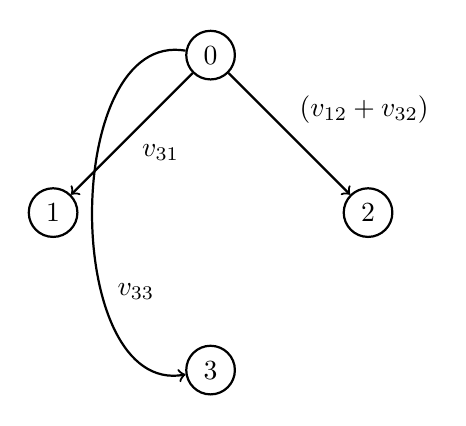
\begin{tikzpicture}[node distance={10mm}, thick, main/.style = {draw, circle}] 
    \node[main] (1) at (0,0) {$0$};
    \node[main] (2) at (-2,-2) {$1$};
    \node[main] (3) at ( 2,-2) {$2$};
    \node[main] (4) at (0,-4) {$3$};

    \draw[->] (1) -- node[midway, below right]{$v_{31}$} (2);
    \draw[->] (1) -- node[midway, above right]{$(v_{12}+v_{32})$} (3);
    \draw[->] (1) edge [bend right = 100] node[midway, above right, pos = 0.7]{$v_{33}$} (4);
    \end{tikzpicture} 
    \caption{$\Gamma_{3,1}$ after isolation.}
  \end{subfigure} 
  \hspace{6em}
  \begin{subfigure}[b]{0.25\textwidth}
  \centering
    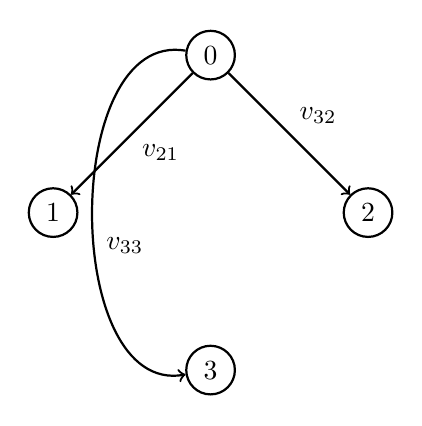
\begin{tikzpicture}[node distance={10mm}, thick, main/.style = {draw, circle}] 
    \node[main] (1) at (0,0) {$0$};
    \node[main] (2) at (-2,-2) {$1$};
    \node[main] (3) at ( 2,-2) {$2$};
    \node[main] (4) at (0,-4) {$3$};

    \draw[->] (1) -- node[midway, below right]{$v_{21}$} (2);
    \draw[->] (1) -- node[midway, above right]{$v_{32}$} (3);
    \draw[->] (1) edge [bend right = 100] node[midway, above right, pos = 0.6]{$v_{33}$} (4);

    \end{tikzpicture} 
    \caption{$\Gamma_{3,2}$ after isolation.}
    \end{subfigure}

    \caption{Fully isolated $\Gamma_3$ digraphs.  (a) $W(B) = v_{31}(v_{12}+v_{32})v_{33}$.  (b) $W(B) = v_{21}v_{32}v_{33}$.} \label{fig:g3}
\end{figure}

The sum of all the arborescence weights is given by the following equation which, when expanded, is equal to the determinant of the matrix given by Eq. \ref{eq:example_det}

\begin{equation}
\begin{split}
    \sum_B W(B) &= v_{11}\left[(v_{12}+v_{22})(v_{13}+v_{23}+v_{33}) + v_{32}(v_{13}+v_{33})\right] \\ 
    &+ v_{22} \left[(v_{21}+v_{31})(v_{33} + v_{23}) + v_{21}v_{13}\right]\\ 
    &+ v_{33}\left[v_{31}(v_{12}+v_{32}) + v_{21}v_{32}\right]
\end{split}
\end{equation}

 \section{Factoring by Explicit Rooting Example}. 

One may factor by explicitly rooting at combinations of vertices.  For an $N$ vertex graph (plus one root 0), there are $2^N - 1$ such rootings.  One can isolate the rooted vertices and explicitly root again until all vertices are isolated.

Consider the $3 \times 3$ matrix of Eq. (\ref{eq:A}) and its matrix digraph in Fig. \ref{fig:3digraph}.  There are seven explicit rootings.  After fully isolating the vertices, the resulting terms in the branching sums are:

{\bf Root at 1}: $\Sigma_1 = v_{11} \left(v_{12} v_{13} + v_{12} v_{23} + v_{13} v_{32}\right)$

{\bf Root at 1 and 2}: $\Sigma_{12} = v_{11} v_{22} \left( v_{13} + v_{23}\right)$

{\bf Root at 1 and 3}: $\Sigma_{13} = v_{11} v_{33} \left( v_{12} + v_{32}\right)$

{\bf Root at 1, 2, and 3}: $\Sigma_{123} = v_{11} v_{22} v_{33}$

{\bf Root at 2}: $\Sigma_2 = v_{22} \left(v_{21} v_{23} + v_{21} v_{13} + v_{23} v_{31}\right)$

{\bf Root at 2 and 3}: $\Sigma_{23} = v_{22} v_{33} \left(v_{21} + v_{31}\right)$

{\bf Root at 3}: $\Sigma_3 = v_{33} \left(v_{31} v_{32} + v_{31} v_{12} + v_{32} v_{21}\right)$

The determinant is the combination of these terms; thus, one factoring could be

\begin{equation}
    \begin{split}
    det(A) = \Sigma_1 + \Sigma_{12} + \Sigma_{13} + \Sigma_{123} + \Sigma_2 + \Sigma_{23} + \Sigma_3 \\
    = v_{11} [\left(v_{12} v_{13} + v_{12} v_{23} + v_{13} v_{32}\right) + v_{22} \left(v_{13} + v_{23}\right) + v_{33} \left(v_{12} + v_{32}\right) + v_{22} v_{33}]+\\
    v_{22} [\left(v_{21} v_{23} + v_{21} v_{13} + v_{23} v_{31}\right) + v_{33} \left(v_{21} + v_{31}\right)] + v_{33} [v_{31} v_{32} + v_{31} v_{12} + v_{32} v_{21}]
    \end{split}
\end{equation}

Alternatively, apportion the terms equally among the rooted vertices to obtain a symmetrical factoring:

\begin{equation}
    \begin{split}
    det(A) = \\
    v_{11}[\left(v_{12} v_{13} + v_{12} v_{23} + v_{13} v_{32}\right) + \frac{1}{2} v_{22} \left(v_{13} + v_{23}\right) + \frac{1}{2} v_{33} \left(v_{12} + v_{32}\right) + \frac{1}{3} v_{22} v_{33}] \\
    +v_{22}[\left(v_{21} v_{23} + v_{21} v_{13} + v_{23} v_{31}\right) + \frac{1}{2} v_{11} \left(v_{13} + v_{23}\right) + \frac{1}{2} v_{33} \left(v_{21} + v_{31}\right) + \frac{1}{3} v_{11} v_{33}] \\
    +v_{33}[\left(v_{31} v_{32} + v_{31} v_{12} + v_{32} v_{21}\right) + \frac{1}{2} v_{11} \left(v_{12} + v_{32}\right) + \frac{1}{2} v_{22} \left(v_{21} + v_{31}\right) + \frac{1}{3} v_{11} v_{33}]
    \end{split}
\end{equation}

\end{document}


